\documentclass{article}
\usepackage[utf8]{inputenc}
\usepackage{amsmath}
\usepackage{systeme}
\usepackage{amssymb}
\usepackage[most]{tcolorbox}
\usepackage[scale=.95,type1]{cabin}
\usepackage{lmodern}

\usepackage{float}
\usepackage{graphicx}

\usepackage[legalpaper,margin=1in]{geometry}

\setlength{\parindent}{10pt}
\setlength{\parskip}{1em}
\renewcommand{\baselinestretch}{1.2}

\title{Vector Spaces}
\date{}

\newcounter{example}[section]
\newenvironment{example}[1][]{\refstepcounter{example}\par\medskip
   \noindent \textbf{Example~\theexample. #1} \rmfamily}{\medskip}

\makeatletter
\renewcommand*\env@matrix[1][*\c@MaxMatrixCols c]{%
  \hskip -\arraycolsep
  \let\@ifnextchar\new@ifnextchar
  \array{#1}}
\makeatother

\newcommand\y{\cellcolor{blue!10}}
\newcommand\B{\textbf}
\newcommand\tcl{\begin{tcolorbox}[colback = {blue9}]}
\newcommand\etcl{\end{tcolorbox}}

\usepackage{tabularray}
\SetTblrInner{colsep=5pt,rowsep=1pt}

\newcommand\x{\times}
\newcommand\xor{\oplus}

\makeatletter
\newcommand{\dashover}[2][\mathop]{#1{\mathpalette\df@over{{\dashfill}{#2}}}}
\newcommand{\fillover}[2][\mathop]{#1{\mathpalette\df@over{{\solidfill}{#2}}}}
\newcommand{\df@over}[2]{\df@@over#1#2}
\newcommand\df@@over[3]{%
  \vbox{
    \offinterlineskip
    \ialign{##\cr
      #2{#1}\cr
      \noalign{\kern1pt}
      $\m@th#1#3$\cr
    }
  }%
}
\newcommand{\dashfill}[1]{%
  \kern-.5pt
  \xleaders\hbox{\kern.5pt\vrule height.4pt width \dash@width{#1}\kern.5pt}\hfill
  \kern-.5pt
}
\newcommand{\dash@width}[1]{%
  \ifx#1\displaystyle
    2pt
  \else
    \ifx#1\textstyle
      1.5pt
    \else
      \ifx#1\scriptstyle
        1.25pt
      \else
        \ifx#1\scriptscriptstyle
          1pt
        \fi
      \fi
    \fi
  \fi
}
\newcommand{\solidfill}[1]{\leaders\hrule\hfill}
\makeatother

\newcommand\R{\mathbb{R}}
\newcommand\T{\textit}
\usepackage{mathtools}

\DeclarePairedDelimiter\abs{\lvert}{\rvert}%
\DeclarePairedDelimiter\norm{\lVert}{\rVert}%

% Swap the definition of \abs* and \norm*, so that \abs
% and \norm resizes the size of the brackets, and the 
% starred version does not.
\makeatletter
\let\oldabs\abs
\def\abs{\@ifstar{\oldabs}{\oldabs*}}
%
\let\oldnorm\norm
\def\norm{\@ifstar{\oldnorm}{\oldnorm*}}
\makeatother

\newcommand*{\Value}{\frac{1}{2}x^2}%
\newcommand\la{\langle}
\newcommand\ra{\rangle}

\begin{document}

    \section{Length and Dot Product in $\R^n$}
        
    \subsection{Reviewing $\R^2$}
    If $\B{v} = (v_1, v_2)$, then \B{length} (or \B{magnitute}) of \B{v} is
    \[ ||\B{v}|| = \sqrt{v_1^2 + v_2^2}\]

    \tcl
        \B{Length of a Vector in $\R^n$}
            The \B{length}, or \B{magnitute} of a vector \B{v}$ = (v_1, v_2, \dots, v_n)$ in $\R^n$ is 
            \[ ||\B{v}|| = \sqrt{v_1^2 + v_2^2 +  \dots + v_n^2}\]
    \etcl 
    \B{REMARK. } The length of a vector is also called its \B{norm}. If $||\B{v}|| = 1$, then \B{v}
    is a \B{unit vector}.
    \begin{center}
        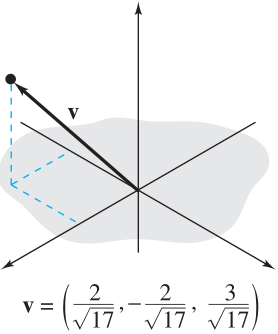
\includegraphics[width = 5cm]{images/lengthr3.png}
    \end{center}
    Each vector in the \T{standard basis} for $\R^n$ has length $1$ and is called \B{standard unit vector}
    in $\R^n$. 2 vectors are \T{parallel} if one is a scalar multiple of the other.
    
    \tcl
        \B{Length of a Scalar Multiple. }
        \[ ||c\B{v}|| = |c|.||\B{v}||\]
    \etcl 

    \tcl
    \T{THEOREM 5.2} \B{Unit Vector in the Direction of v. } If \B{v} is a nonzero vector in $\R^n$, then
    \[\B{u} = \frac{\B{v}}{||\B{v}||} \]
    is the \B{unit vector in the direction of v} \T{(has length $1$ and same direction as \B{v})}.
    \etcl 

    \B{Example 2. } Finding a Unit Vector for \B{v}$ = (3, -1, 2)$.
    \begin{center}
        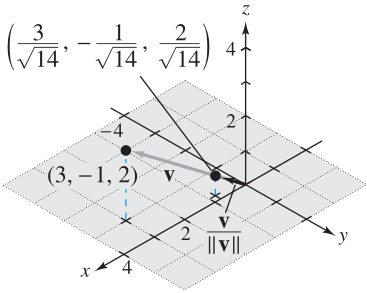
\includegraphics[width = 5cm]{images/egunitv.png}
    \end{center}
    
    \subsection{Distance Between 2 Vectors in $\R^n$}

    \B{$\R^2$ as a model.}\\ 
    $\quad$The distance between 2 point $\B{u} = (u_1, u_2)$ and $\B{v} = (v_1, v_2)$ is $d = \sqrt{(u_1 - v_1)^2 + (u_2 - v^2)^2}$.
    \begin{center}
        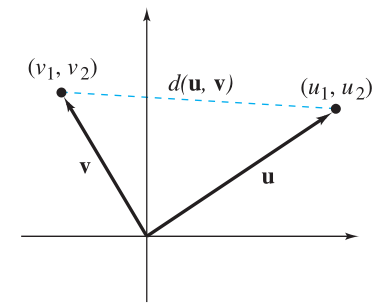
\includegraphics[width = 5cm]{images/r2dis.png}
    \end{center}

    \tcl
    \B{Distance Between 2 Vectors. } The \B{distance between 2 vectors u} and \B{v } in $\R^n$ is
    \[ d(\B{u}, \B{v}) = ||\B{u} - \B{v}|| \]
    \etcl 

    \subsection{Dot Product and the Angle Between 2 Vectors}

    
    \begin{minipage}{0.3\textwidth}
    \begin{figure}[H]
    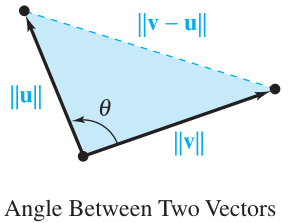
\includegraphics[width = 4cm]{images/angleuv.png}
    \end{figure}
    \end{minipage} 
    \begin{minipage}{0.65\textwidth}
        To find the angle $\theta (0 \le \theta \le \pi)$ of 2 vectors in $\R^2$, the \T{Law of Cosines} can be applied 
        \[  ||\B{v} - \B{u}||^2 = ||\B{u}||^2 + ||\B{v}||^2 - 2\norm{\B{u}}\norm{\B{v}}\cos{\theta}\]
        Expanding and solving for $\cos{\theta}$ yields
        \[ \cos{\theta} = \frac{u_1v_1 + u_2v_2}{\norm{\B{u}}\norm{\B{v}}}\]
    \end{minipage}

    The numerator of the quotient above is defined as the \B{dot product} of \B{u} and \B{v} 
    \[ \B{u} \cdot \B{v} = u_1v_1 + u_2v_2 \]

    \tcl
        \B{Dot Product in $\R^n$. } The \B{dot product} of \B{u} and \B{v} is the \T{scalar} quantity
        \[\B{u} \cdot \B{v} = u_1v_1 + u_2v_2 + \cdots + u_nv_n \]
    \etcl 
    \B{Notice. } The dot product of 2 vectors is a \T{scalar}, not another vector.

    \tcl
    \T{THEOREM 5.3 } \B{Properties of the Dot Product}
    \begin{enumerate}
        \item $\B{u} \cdot \B{v} = \B{v} \cdot \B{u}$
        \item $\B{u} \cdot (\B{v} + \B{w}) = \B{u} \cdot \B{v} + \B{u} \cdot \B{w}$
        \item $(\B{u} \cdot \B{v}) = (c\B{u}) \cdot \B{v} = \B{u} \cdot (c\B{v}) $
        \item $\B{v} \cdot \B{v} = \norm{v}^2$
        \item $\B{v} \cdot \B{v} \ge 0$, $\B{v} \cdot \B{v} = 0$ if and only if $\B{v} = 0$.
    \end{enumerate}
    \etcl 
    


    \tcl
        \T{THEOREM 5.4 } \B{The Cauchy-Schwarz Inequality}

        If \B{u} and \B{v} are vectors in $\R^n$, then 
        \[ |\B{u} \cdot \B{v} | \le \norm{\B{u}} \norm{\B{v}},\]
        wher $|\B{u} \cdot \B{v}|$ denotes the \T{absolute value} of $\B{u} \cdot \B{v}$.
    \etcl 

    \tcl 
    \B{The Angle Between 2 Vectors in $\R^n$.}
    The angle $\theta$ between 2 nonzero vectors \B{u} and \B{v} in $\R^n$, 
    \[ \cos{\theta} = \frac{\B{u} \cdot \B{v}}{\norm{\B{u}} \norm{\B{v}}}, \quad 0 \le \theta \le \pi \]
    \etcl 

    \B{Example. } The angle between \B{u}$ = (-4, 0, 2, -2)$ and $\B{v} = (2, 0, -1, 1)$ is
    \[ \cos{\theta} = \frac{\B{u} \cdot \B{v}}{\norm{\B{u}} \norm{\B{v}}} = -\frac{12}{\sqrt{24} \sqrt{6}} = -1 \]
    Consequently, $\theta = \pi$. It makes sense that \B{u} and \B{v} should have opposite direction,
    because $\B{u} = -2\B{v}$.

    \B{Note. }  Because \B{u} and \B{v} are always positive, $\B{u} \cdot \B{v}$ and $\cos{\theta}$ will always
    have the same sign. The sign of the \T{dot product} can be used to determine whether $\theta$ is
    \T{acute} or \T{obtuse}.
    \begin{center}
        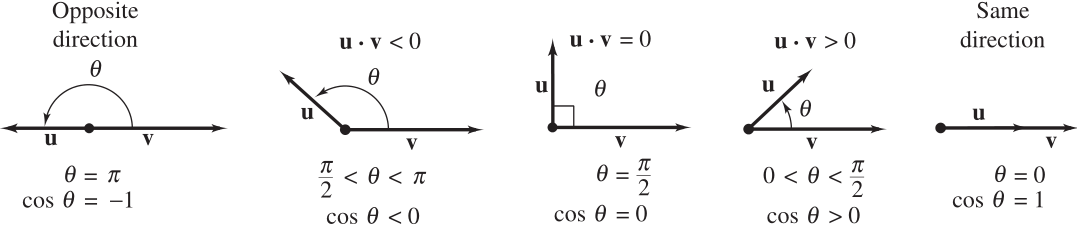
\includegraphics[width = 13cm]{images/angleacute.png}
    \end{center}

    \tcl
    \B{Orthogonal Vectors. } Two vectors \B{u} and \B{v} in $\R^n$ are \B{orthogonal} (or \T{perpendicular})
    if \[ \B{u} \cdot \B{v} = 0 \]
    \etcl 
    \B{REMARK. } The vector \B{0} is orthogonal to every vector.

    \B{Example. } Finding Orthogonal Vectors.
    
    Determine all vectors in $\R^2$ that are orthogonal to \B{u}$ = (4, 2)$.

    \begin{minipage}{0.3\textwidth}
    \begin{figure}[H]
    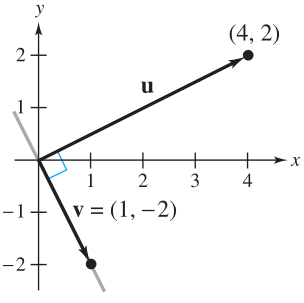
\includegraphics[width = 4cm]{images/42eg.png}
    \end{figure}
    \end{minipage} 
    \begin{minipage}{0.65\textwidth}
    \T{SOLUTION. } Let \B{v}$ = (v_1, v_2)$ be orthogonal to \B{u}. Then
    \[ \B{u} \cdot \B{v} = 4v_1 + 2v_2 = 0\]
    which implies that $2v_2 = -4v_1$ and $v_2 = -2v_1$. So every vector that is orthogonal to $(4, 2)$ is 
    of the form 
    \[ \B{v} = (t, -2t) = t(1, -2)\]
    where $t$ is a real number.

    \end{minipage}

    \tcl
    \T{THEOREM 5.5 } \B{The Triangle Inequality}
    
    If \B{u} and \B{v} are vectors in $\R^n$, then
    \[ \norm{\B{u} + \B{v}} \le \norm{\B{u}} + \norm{\B{v}} \]
    \etcl 
    \begin{center}
        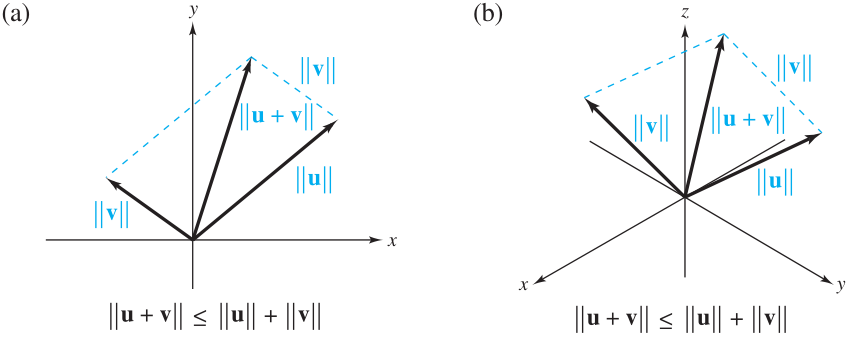
\includegraphics[width = 11cm]{images/triangleine.png}
    \end{center}
    \B{REMARK. } Equality occurs in the Triangle Inequality if and only if \B{u} and \B{v} have the same
    direction.
    \tcl
    \T{THEOREM 5.6} \B{The Pythagorean Theorem}

    If \B{u} and \B{v} are vectors in $\R^n$, then they are orthogonal if and only if
    \[ \norm{\B{u} + \B{v}}^2 = \norm{\B{u}}^2 + \norm{\B{v}}^2\]
    \etcl 
    \B{\T{Proof. }}  $\norm{\B{u} + \B{v}}^2 = \norm{\B{u}}^2 + \norm{\B{v}}^2 + 2(\B{u} \cdot \B{v})$, and their dot
    product is zero.

    \subsection{The Dot Product and Matrix Multiplication}

    Let $\B{u} = 
    \begin{bmatrix}
        u_1 \\ u_2 \\ \vdots \\ u_n 
    \end{bmatrix}, \quad  \B{v} =
    \begin{bmatrix}
        v_1 \\ v_2 \\ \vdots \\ v_n
    \end{bmatrix}$. Then the \B{dot product} of 2 vectors is 
    \[ \B{u} \cdot \B{v} = \B{u}^T\B{v} = 
        \begin{bmatrix}
            u_1 & u_2 & \cdots & u_n 
        \end{bmatrix} 
        \begin{bmatrix}
            v_1 \\ v_2 \\ \vdots \\ v_n 
        \end{bmatrix} =
        \begin{bmatrix}
            u_1v_1 + u_2v_2 + \cdots + u_3v_3
        \end{bmatrix}\]
    
    \section{Inner Product Spaces}

    The previous \textit{dot product} in $\R^n$ is an example of \B{inner product} -  called \B{Euclidean inner product}.
    To distinguish between the standard inner product and other possible inner products,
    \[\B{u} \cdot \B{v} = \text{dot product (Euclidean inner product for $\R^n$)}\]
    \[ \la \B{u} \cdot \B{v} \ra = \text{general inner product for vector space $V$}\]

    \tcl
    \B{Inner Product. } Let \B{u}, \B{v} and \B{w} be vectors in $V$. An \textbf{inner product} on $V$ is a function that
    associates a real numer $\la \B{u} \cdot \B{v} \ra$ with each pair of (\B{u}, \B{v}) satisfies these axioms.
    \begin{enumerate}
        \item $\la \B{u} \cdot \B{v} \ra = \la \B{v} \cdot \B{u} \ra$
        \item $\la \B{u} \cdot \B{v + w} \ra = \la \B{u} \cdot \B{v} \ra + \la \B{u} \cdot \B{w} \ra$
        \item $c\la \B{u} \cdot \B{v} \ra = \la c\B{u} \cdot \B{v} \ra$
        \item $\la \B{v} \cdot \B{v} \ra \ge 0$, and $\la \B{v} \cdot \B{v} \ra = 0$ if and only if $\B{v} = \B{0}$.
    \end{enumerate}
    \etcl 
    \B{REMARK. } A vector space $V$ with an inner product is called an \B{inner product space}.

    (1) \B{A Different Inner Product for $\R^2$}

    Show that the following function defines an inner product on $\R^2$
    \[ \la \B{u} \cdot \B{v} \ra = u_1v_1 + 2u_2v_2 \]
    This example can be generalize to show that
    \[ \la \B{u} \cdot \B{v} \ra = c_1u_1v_1 + c_2u_2v_2 + \cdots + c_nu_nv_n, \quad c_i > 0 \]
    is an inner product of $\R^n$. The positive constants $c_1, c_2, \dots, c_n$ are \B{weights}. If any $c_i \le 0$,
    then this function does not define an inner product.
    
    (2) \B{A Function That is Not an Inner Product}
    \[ \la \B{u} \cdot \B{v} \ra = u_1v_1 - 2u_2v_2 + u_3v_3 \]

    (3) \B{An Inner Product on $M_{2,2}$}

    Let $A = 
        \begin{bmatrix}
            a_{11} & a_{12} \\
            a_{21} & a_{22}
        \end{bmatrix}, \quad \text{and} \quad 
        B =
        \begin{bmatrix}
            b_{11} & b_{12} \\
            b_{21} & b_{22}
        \end{bmatrix}$ be matrices in the vector space $M_{2,2}$. 

        The function
        $ \la A, B \ra = a_{11}b_{11} + a_{21}b_{21} + a_{12}b_{12} + a_{22}b_{22}$ is an inner product on $M_{2,2}$.

    (4) \B{An Inner Product Defined by a Definite Integral (Calculus)}
    
    Let $f$ and $g$ be real-valued continuous function in the vector space $C[a,b]$.  Show that
    \[ \la f, g \ra = \int_a^b f(x)g(x) \,dx  \]
    defines an inner product on $C[a,b]$.

    \tcl
    \T{THEOREM 5.7 } \B{Properties of Inner Product}

    Let \B{u}, \B{v} and \B{w} be vectors in an inner product space $V$, and $c \in \R$.
    \begin{enumerate}
        \item $\la \B{0}, \B{v} \ra = \la \B{v}, \B{0} \ra = 0$
        \item $\la \B{u + v}, \B{w} \ra = \la \B{u}, \B{w} \ra +  \la \B{v}, \B{w} \ra $
        \item $ \la \B{u}, c\B{v} \ra = c\la \B{u}, \B{v} \ra$
    \end{enumerate}
    \etcl 

    \tcl
    \B{Definition of Norm, Distance, and Angle.}

    Let \B{u} and \B{v} be vectors in an inner product space $V$.
    \begin{enumerate}
        \item The \B{norm} (or \B{length}) of \B{u} is $\| u \| = \sqrt{\la \B{u}, \B{u} \ra}$.
        \item The \B{distance} between \B{u} amd \B{v} is $d(\B{u}, \B{v}) = \| \B{u} - \B{v} \|$.
        \item The \B{angle} between 2 nonzero vectors \B{u} and \B{v} is given by
            \[ \cos{\theta} = \frac{\la \B{u}, \B{v} \ra }{\|\B{u}\| \|\B{v}\|}, \quad 0 \le \theta \le \pi \]
        \item \B{u} and \B{v} are \B{orthogonal} if $\la \B{u}, \B{v} \ra = 0$.
    \end{enumerate}
    \etcl 
    \B{REMARK. } If $\| \B{v}  \| = 1$, then \B{v} is called a \B{unit vector}. Moreover, $\B{u} = \frac{\B{v}}{\| \B{v} \|}$
    is the \B{unit vector in the direction of v}.
    
    (6) \B{Finding Inner Products}

    For polynomials $p = a_0 + a_1x + \cdots + a_nx^n$ and $q = b_0 + b_1x + \cdots + b_nx^n$ in the vector space $P_n$.
    
    The fuction  $ \la p, q \ra = a_0b_0 + a_1b_1 + \cdots + a_nb_n $ is an inner product.

    \B{Note.} Orthogonality depends on the particular inner product used. That is, 2 vectors may be 
    orthogonal with respect to one inner product but not to another.

    \B{Example 7. Using Inner Product on $C[0,1]$ (Calculus)} (p.316)
    \begin{center}
        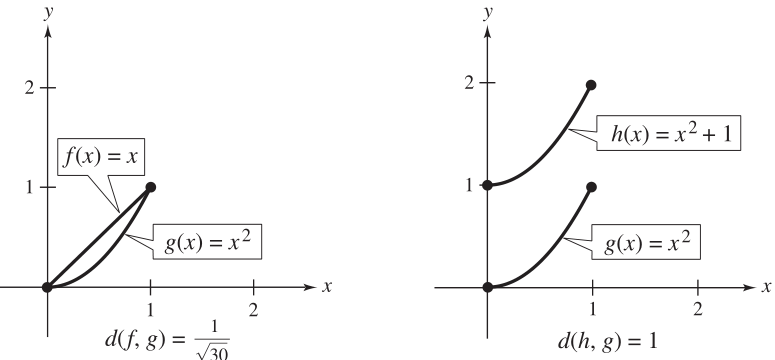
\includegraphics[width = 9cm]{images/disint.png}
    \end{center}
    
    If \B{u} and \B{v} are vectors in an inner product space, then
    \begin{center}
        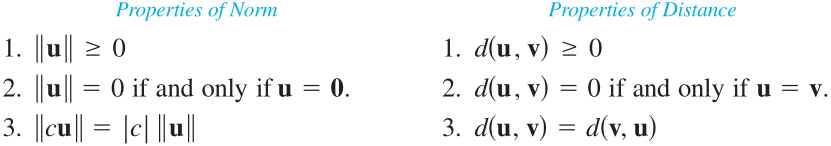
\includegraphics[width = 11cm]{images/sumaryinner.png}
    \end{center}
    \tcl
    \T{THEOREM 5.8 } 
    \begin{enumerate}
        \item Cauchy-Schwarz Inequality: $| \la \B{u}, \B{v} \ra | \le \| \B{u} \| \|\B{v}\|$
        \item Triangle Inequality: $\| \B{u} + \B{v} \| \le \| \B{u} \| + \| \B{v} \|$
        \item Pythagorean Theorem: \B{u} and \B{v} are orthogonal if and only if
            \[ \| \B{u + v} \| = \| \B{u} \|^2 + \| \B{v} \|^2 \]
    \end{enumerate}
    \etcl 

    \subsection{Orthogonal Projections in Inner Product Spaces}

    Let \B{u} and \B{v} be vectors in the plane. If \B{v} is nonzero, then \B{u} can be orthogonally
    projected onto \B{v}. This projection is denoted by 
    \[ \text{proj}_v{\B{u}} = a\B{v}\]
    
    If $a > 0$, then $\cos{\theta} > 0$ and the length of $\text{proj}_v\B{u}$ is
    \[ \| a\B{v} \| = a\|\B{v}\| = \|\B{u}\| \cos{\theta} = \frac{\|\B{u}\| \|\B{v}\|\cos{\theta}}{\|\B{v}\|} = \frac{\B{u} \cdot \B{v}}{\|\B{v}\|}\]
    which implies that $ a = (\B{u} \cdot \B{v})/ \| \B{v} \|^2 = (\B{u} \cdot \B{v})/(\B{v} \cdot \B{v})$. So
    \[ \text{proj}_{\text{v}} \B{u} = \frac{\B{u} \cdot \B{v}}{\B{v} \cdot \B{v}} \B{v}\]
    If $a < 0$, we obtain the same formula. 
    \begin{center}
        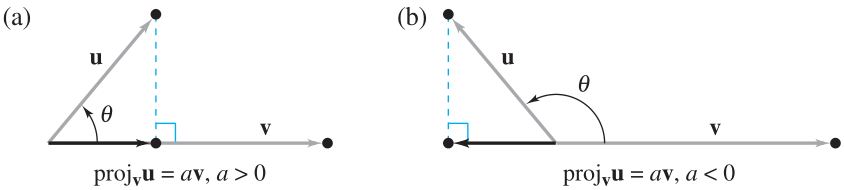
\includegraphics[width = 12cm]{images/proj.png}
    \end{center}

    \tcl
    \B{Definition of Orthogonal Projection.} Let \B{u} and \B{v}$ \ne 0$ be vectors in an inner product space $V$,
    then the \B{orthogonal projection} of \B{u} onto \B{v} is
    \[ \text{proj}_{\text{v}}\B{u} = \frac{\la \B{u}, \B{v} \ra}{\la \B{v}, \B{v} \ra} \B{v}\]
    \etcl 
    \B{REMARK. } If \B{v} is an unit vector, then $\la \B{v}, \B{v} \ra = \| \B{v} \|^2 = 1$. The formula takes the
    simpler form \[ \text{proj}_{\text{v}}\B{u} = \la \B{u}, \B{v} \ra \B{v} \]
    
    \begin{minipage}{0.35\textwidth}
    \begin{figure}[H]
    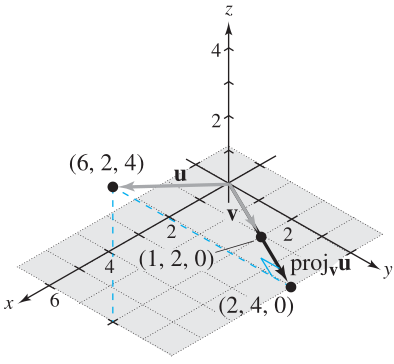
\includegraphics[width = 5cm]{images/projr3.png}
    \end{figure}
    \end{minipage} 
    \begin{minipage}{0.5\textwidth}
        \B{REMARK. } \B{u} - $\text{proj}_\text{v}\B{u}$ is orthogonal to \B{v}. 

        Of all possible scalar multiples of \B{v}, the orthogonal projection of \B{u} onto \B{v} is the one
        \T{closest} to \B{u}.
    \end{minipage}
    \tcl
    \T{THEOREM 5.9} \B{Orthogonal Projection and Distance}

    Let \B{u} and \B{v}$ \ne 0$ be 2 vectors in an inner product space $V$, then
    \[ d(\B{u}, \text{proj}_\text{v}\B{u}) < d(\B{u}, c\B{v}), \quad c \ne \frac{\la \B{u}, \B{v} \ra}{\la \B{v}, \B{v} \ra}\]
    \etcl 
    \begin{center}
        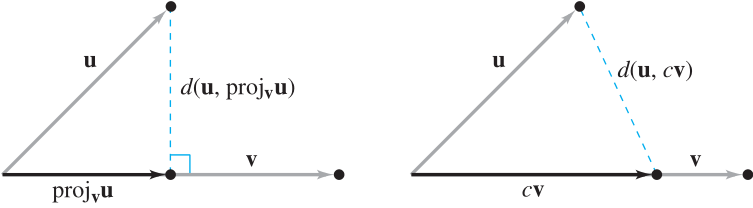
\includegraphics[width = 9cm]{images/projclosest.png}
    \end{center}

    \section{Orthonormal Bases: Gram-Schmidt Process}

    A vector space can have many different bases, but certain bases are more \textit{convenient} than others.
    For example, $\R^3$ has the convenient standard basis $B = \{ (1,0,0), (0,1,0), (0,0,1) \}$. It has 
    special characteristics that are particularly useful. First, 3 vectors in the basis are 
    \textit{mutually orthogonal}. Second, they are all \T{unit} vector.

    \tcl
    \B{Definition of Orthogonal and Orthonormal Sets}

    A set $S$ of vectors in an inner product space $V$ is \B{orthogonal} if every pair of
    vectors in $S$ is orthogonal. If, in addition, each vector in the set is a \T{unit} vector,
    then $S$ is \B{orthonormal}.
    \etcl 

    \begin{minipage}{0.35\textwidth}
    \begin{figure}[H]
    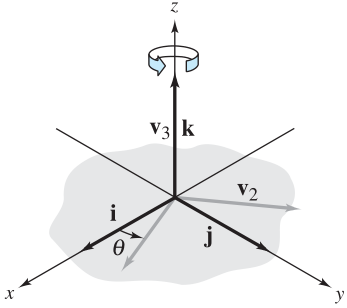
\includegraphics[width = 5cm]{images/r3rotatebasis.png}
    \end{figure}
    \end{minipage} 
    \begin{minipage}{0.6\textwidth}
        If $S$ is a \textit{basis}, then it is called an \B{orthogonal basis} or 
        an \B{orthonormal basis}, respectively.

        The standard basis for $\R^n$ is orthonormal, but it is not the only one. For instance,
        rotating the standard basis in $\R^3$ about the $z$-axis to form
        \[B = \{ (\cos{\theta}, \sin{\theta},0), (-\sin{\theta}, \cos{\theta}, 0), (0, 0, 1) \} \]
    \end{minipage}

    \begin{minipage}{0.6\linewidth}
        \B{A Nonstandard Orthonormal Basis for $\R^3$}
        \[S = \left\{ \left( \frac{1}{\sqrt{2}}, \frac{1}{\sqrt{2}}, 0 \right), \left( -\frac{\sqrt{2}}{6}, \frac{\sqrt{2}}{6},\frac{2\sqrt{2}}{3} \right),
                \left( \frac{2}{3}, -\frac{2}{3}, \frac{1}{3} \right) \right\} \]
        3 vectors are \T{mutually orthogonal}. Each vector is of length $1$.
    \end{minipage}
    \begin{minipage}{0.35\linewidth}
        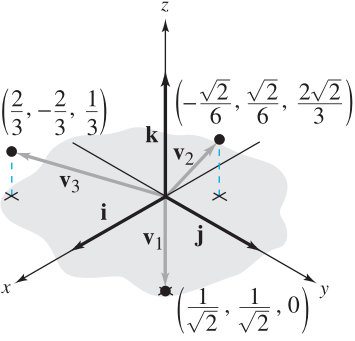
\includegraphics[width = 5cm]{images/r3nonstan.png}
    \end{minipage}

    \tcl
    \T{THEOREM 5.10} \B{Orthogonal Sets Are Linearly Independent}

    If $S = \{ \B{v}_1, \B{v}_2, \dots, \B{v}_n \}$ is an orthogonal set of nonzero vectors in an inner product
    space $V$, then $S$ is \textit{linearly independent}.
    \etcl 

    \tcl
    \T{COROLLARY TO THEOREM 5.10} 

    If $V$ is an inner profuct space of dimension $n$, then any orthogonal set of $n$ nonzero vectors is a
    basis for $V$.
    \etcl 

    \begin{center}
        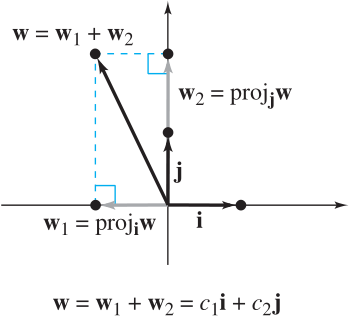
\includegraphics[width = 5cm]{images/coordinateorthonormal.png}
    \end{center}
    \tcl
    \T{THEOREM 5.11} \B{Coordinates Relative to an Orthonormal Basis}

    If $B = \{ \B{v}_1, \B{v}_2, \dots, \B{v}_n\}$ is an \textit{orthonormal} basis for an inner product space $V$, then
    the coordinate representation of a vector \B{w} with respect to $B$ is
    \[ \B{w} = \la \B{w}, \B{v}_1 \ra \B{v}_1 + \la \B{w}, \B{v}_2 \ra \B{v}_2 + \cdots 
        + \la \B{w}, \B{v}_n \ra \B{v}_n \]
    \etcl 
    The coordinates of \B{w} relative to the \T{orthonormal} basis $B$ are called the \B{Fourier coefficents}
    of \B{w} relative to $B$. The corresponding coordinate matrix of \B{w} relative to $B$ is
    \[ [\B{w}]_B = 
        \begin{bmatrix}
            c_1 \\ c_2 \\ \vdots \\ c_n
        \end{bmatrix}
        = \begin{bmatrix}
            \la \B{w}, \B{v}_1 \ra \\
            \la \B{w}, \B{v}_2 \ra \\
            \vdots \\
            \la \B{w}, \B{v}_n \ra
        \end{bmatrix} \]

    \subsection{Gram-Schmidt Orthonormalization Process}

    One of the advantages of orthonormal bases is the \B{straighforwardness} of coordinate representation.
    We will now look at a procedure called the \B{Gram-Schmidt orthonormalization process} to find such
    a basis. 

    It has three steps.
    \begin{enumerate}
        \item Begin with a basis for the inner prodcut space. (no need to be orthorgonal nor orthonormal)
        \item Convert the basis to an orthogonal basis.
        \item Normalize each vector to form an orthonormal basis.
    \end{enumerate}
    \B{REMARK. } This process leads to a matrix factorization similar to the $LU$-factorization.\\
    The \textbf{\textit{QR}-factorization} is in \T{Project 1}.

    \tcl
        \T{THEOREM 5.12} \B{Gram-Schmidt Orthonormalization Process}
        \begin{enumerate}
            \item Let $B = \{ \B{v}_1, \B{v}_2, \dots, \B{v}_n \}$ be a basis for an inner product space $V$.
            \item Let $B' = \{ \B{w}_1, \B{w}_2, \dots, \B{w}_n \}$, where $\B{w}_i$ is given by
                \begin{equation*}
                    \begin{split}
                        \B{w}_1 & = \B{v}_1 \\
                        \B{w}_2 & = \B{v}_2 - \frac{\la \B{v}_2, \B{w}_1\ra}{\la \B{w}_1, \B{w}_1\ra} \B{w}_1\\
                        \B{w}_3 & = \B{v}_3 - \frac{\la \B{v}_3, \B{w}_1\ra}{\la \B{w}_1, \B{w}_1\ra} \B{w}_1
                        - \frac{\la \B{v}_3, \B{w}_2\ra}{\la \B{w}_2, \B{w}_2\ra} \B{w}_2 \\
                                & \vdots \\
                        \B{w}_n & = \B{w}_n - \frac{\la \B{v}_n, \B{w}_1\ra}{\la \B{w}_1, \B{w}_1\ra} \B{w}_1
                        - \frac{\la \B{v}_n, \B{w}_2\ra}{\la \B{w}_2, \B{w}_2\ra} \B{w}_2  - \cdots 
                        - \frac{\la \B{v}_n, \B{w}_{n-1}\ra}{\la \B{w}_{n-1}, \B{w}_{n-1}\ra} \B{w}_{n-1}
                    \end{split}
                \end{equation*}
            \item Let $\B{u}_i = \frac{\B{w}_i}{\| \B{w}_i \|}$. Then the set $B'' = \{ \B{u}_1, \B{u}_2, \dots, \B{u}_n \}$
                is an \T{orthonormal} basis for $V$. 

                Moreover, span $\{ \B{v}_1, \B{v}_2, \dots, \B{v}_k \} =$
                span $\{ \B{u}_1, \B{u}_2, \dots, \B{u}_k \}$ for $k = 1, 2, \dots, n$.
        \end{enumerate}
    \etcl 
    \B{REMARK. } An orthonormal set derived by the Gram-Schmidt orthonormalization process depends on
    the \textit{order of the vectors} in the basis.

    This process works equally well for a subspace of an inner product space.

    \B{Example 8. Applying the Gram-Schmidt Orthonormalization Process}

    \begin{minipage}{0.31\linewidth}
        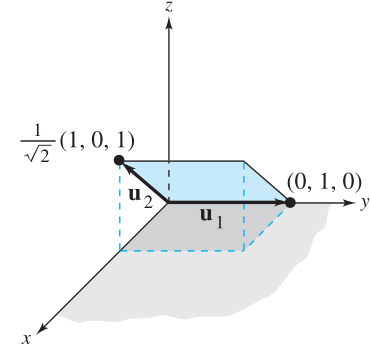
\includegraphics[width = 5cm]{images/gram1.png}
    \end{minipage}
    \begin{minipage}{0.63\linewidth}
        The vectors $\B{v}_1 = (0, 1, 0)$ and $\B{v}_2 = (1, 1, 1)$ span a plane in $\R^3$. Find an orthonormal
        basis for this subspace.

        \T{SOLUTION. } Applying the Gram-Schmidt Orthonormalization Process produces
        $\{ (0, 1, 0), (\frac{\sqrt{2}}{2}, 0, \frac{\sqrt{2}}{2}) \}$.
    \end{minipage}

    \B{Example 9.} Applying the Gram-Schmidt orthonormalization process to the basis $B = \{1, x, x^2\}$ in $P_2$,
    using the inner product 
    \[ \la p, q \ra = \int_{-1}^1 p(x)q(x)\,dx \]
    \T{SOLUTION. } Let $B = \{1, x, x^2 \} = \{ \B{v}_1, \B{v}_2, \B{v}_3 \}$. Then we have
    \begin{equation*}
        \begin{split}
            \B{w}_1 & = \B{v}_1 = 1 \\ 
            \B{w}_2 & = \B{v}_2 - \frac{\la \B{v}_2, \B{w}_1 \ra}{\la \B{w}_1, \B{w}_1\ra}\B{w}_1 = x - \frac{0}{2}(1) = x \\
            \B{w}_3 & = \B{v}_3 - \frac{\la \B{v}_3, \B{w}_1 \ra}{\la \B{w}_1, \B{w}_1\ra}\B{w}_1 -
            \frac{\la \B{v}_3, \B{w}_2 \ra}{\la \B{w}_2, \B{w}_2\ra}\B{w}_2\\
                    & = x^2 - \frac{2/3}{2}(1) - \frac{0}{2/3}(x)\\
                    & = x^2 - \frac{1}{3}
        \end{split} 
    \end{equation*}

    By normalizing these above vectors, we have $B'' = \{ \frac{1}{\sqrt{2}}, \frac{\sqrt{3}}{\sqrt{2}}x, 
        \frac{\sqrt{5}}{2\sqrt{2}}(3x^2 - 1)$.

    \B{REMARK. } The polynomials $\{ \frac{1}{\sqrt{2}}, \frac{\sqrt{3}}{\sqrt{2}}x, 
    \frac{\sqrt{5}}{2\sqrt{2}}(3x^2 - 1)$\} are called the first three \B{normalized
    Legendre polynomials}.

    The computations in the Gram-Schmidt orthonormalization process are sometimes simpler when
    each vector $\B{w}_i$ is normalized \T{before} it is used to determine the next vector.
    \tcl
    \B{The alternative form of the Gram-Schmidt orthonormalization process.}
    \begin{equation*}
        \begin{split}
            \B{w}_1 & = \frac{\B{v}_1}{\| \B{v}_1 \|} \\
            \B{w}_2 & = \frac{\B{w}_2}{\| \B{w}_2 \|}, \text{where } \B{w}_2 = \B{v}_2 - \la \B{v}_2, \B{w}_1\ra \B{w}_1\\
            \B{w}_3 & = \frac{\B{w}_3}{\| \B{w}_3 \|}, \text{where } \B{w}_3 = \B{v}_3 - \la \B{v}_3, \B{w}_1\ra \B{w}_1
            - \la \B{v}_3, \B{w}_2\ra \B{w}_2 \\
                    & \vdots \\
            \B{w}_n & = \frac{\B{w}_n}{\|\B{w}_n\|}, \text{where } \B{w}_n = \B{w}_n - \la \B{v}_n, \B{w}_1\ra \B{w}_1
             - \cdots 
            - \la \B{v}_n, \B{w}_{n-1}\ra \B{w}_{n-1}
        \end{split}
    \end{equation*}
    \etcl 

    \section{Mathematical Models and Least Squares Analysis}
    This section is about \T{inconsistent} systems of linear equations and learn to find the 
    "best possible solution" of such a system.

    \B{Example 1. Least Square Regression Line}

    Look for an \B{x} that \T{minimizes} the norm of the error $\norm{A\B{x} - b}$.\\
    The solution $\B{x} = \begin{bmatrix}
        c_0 \\ c_1 
    \end{bmatrix}$ of this minimization problem is called \B{least square  regression line}
    $y = c_0 + c_1x$.

    To begin, consider $A\B{x} = \B{b}$, where $A$ is an $m \x n$ matrix and \B{b} is a column
    vector in $\R^m$. If the system is \T{consistent}, use Gaussian elimination with 
    back-substitution to solve for \B{x}. If not, however, find the "best possible" solution,
    which difference between $A\B{x}$ and \B{b} is smallest.
    \tcl
    \B{Least Squares Problem. } Given an $m \x n$ matrix $A$ and a vector \B{b} in $\R^m$, find \B{x}
    in $\R^n$ such that $\norm{A\B{x} - \B{b}}^2$ is minimized.
    \etcl 

    \subsection{Orthogonal Subspaces}

    \tcl
    \B{Definition of Orthogonal Subspaces.} 
    
    The subspace $S_1$ and $S_2$ of $\R^n$ are \textbf{orthogonal} if $\B{v}_1 \cdot \B{v}_2 = 0$ for all $\B{v}_1$ in $S_1$ and $\B{v}_2$ in $S_2$.
    \etcl 
    \B{Example 2.} $S_1 = \text{span}\left( 
        \begin{bmatrix}
            1 \\ 0 \\ 1
        \end{bmatrix},
        \begin{bmatrix}
            1 \\ 1 \\ 0
        \end{bmatrix}
        \right) \quad \text{ and   } \quad 
        S_2 = \text{span}\left(
            \begin{bmatrix}
                -1 \\ 1 \\ 1
            \end{bmatrix}
            \right)$
    
    \B{Notice.} The zero vector is the only common vector to both $S_1$ and $S_2$. It's the only intersection.
    \tcl 
    \B{Definition of Orthogonal Complement}

    If $S$ is a subspace of $\R^n$, then the \B{orthogonal complement of \textit{S}} is the set 
    \[ S^{\perp} = \{ \B{u} \in \R^n : \B{v} \cdot \B{u} = 0 \quad \forall \B{v} \in S \} \]
    \etcl 
    The orthogonal complement of the trivial subspace $\{ \B{0} \}$ is all of $\R^n$, and conversely, the 
    orthogonal complement of $\R^n$ is the trivial subspace $\{\B{0}\}$. In general, the orthogonal complement
    of a subspace of $\R^n$ is itself a \textit{subspace} of $\R^n$.

    \B{Example 3. Finding the Orthogonal Complement}

    Find the orthogonal complement of the subspace $S$ of $\R^4$ spanned by 2 column vectors $\B{v}_1$ and $\B{v}_2$
    of the matrix $A$.
    \[ A =
            \underset{\B{v}_1 \quad \B{v}_2}{
            \begin{bmatrix}
                1 & 0 \\ 2 & 0 \\ 1 & 0 \\ 0 & 1
            \end{bmatrix}
            } \]
    \T{SOLUTION.} The orthogonal complement of $S$ consists all the vectors \B{u} such that $A^T\B{u} = \B{0}$.
    \[ \begin{bmatrix}
        1 & 2 & 1 & 0 \\
        0 & 0 & 0 & 1
    \end{bmatrix} 
    \begin{bmatrix}
        x_1 \\ 
        x_2 \\
        x_3\\
        x_4
    \end{bmatrix} = 
    \begin{bmatrix}
        0 \\
        0
    \end{bmatrix}\]
    That is, the orthogonal complement of $S$ is the \textit{nullspace} of $A^T$.
    \[S^\perp = N(A^T)\]
    Using the techniques for solving homogeneous linear systems,you can find that a possible basis for the
    orthogonal complement can consist of the 2 vectors
    \[ \B{u}_1 = 
        \begin{bmatrix}
            -2 \\
            1 \\ 0
            \\ 0
        \end{bmatrix} \quad \text{ and } \quad 
    \B{u}_2 = 
        \begin{bmatrix}
            -1 \\
            0  \\
            1 \\
            0
        \end{bmatrix} \]
    \B{Notice.} $\R^4$ here is split into 2 \textit{subspaces}, $S = \text{span}(\B{v}_1, \B{v}_2)$ and
    $S^\perp = \text{span}(\B{u}_1, \B{u}_2)$. In fact, the 4 vectors $\B{v}_1, \B{v}_2, \B{u}_1$ and $\B{u}_2$ form a basis for
    $\R^4$.
    \tcl
    \B{Definition of Direct Sum.} 

    Let $S_1$ and $S_2$ be 2 \T{subspace} of $\R^n$. If each vector $\B{x} \in \R^n$ can be \textit{uniquely} 
    written as a sum of a vector $\B{s}_1$ from $S_1$ and a vector $\B{s}_2$ from $S_2$, $\B{x} = \B{s}_1 + \B{s}_2$,
    then $\R^n$ is \textbf{direct sum} of $S_1$ and $S_2$.
    \[ \R^n = S_1 \oplus S_2 \]
    \etcl 
    \B{Example. }

    (a) $S_1 = \text{span}\left( 
        \begin{bmatrix}
            1 \\ 0 \\ 1
        \end{bmatrix},
        \begin{bmatrix}
            1 \\ 1 \\ 0
        \end{bmatrix}
        \right) \quad \text{ and   } \quad 
        S_2 = \text{span}\left(
            \begin{bmatrix}
                -1 \\ 1 \\ 1
            \end{bmatrix}
            \right), \quad S_1 \oplus S_2 = \R^2$

    (b) $S = \text{span}\left(
            \begin{bmatrix}
                1 \\
                2 \\
                1 \\
                0
            \end{bmatrix},
            \begin{bmatrix}
                0 \\
                0 \\
                0 \\
                1
            \end{bmatrix}
        \right) \quad \text{and} \quad 
        S^\perp = \text{span}\left(
            \begin{bmatrix}
                -2 \\
                1 \\
                0 \\
                0
            \end{bmatrix},
            \begin{bmatrix}
                -1 \\
                0 \\
                1 \\
                0
            \end{bmatrix}
        \right), \quad S \oplus S^\perp = \R^4$

    \tcl
    \T{THEOREM 5.13} \B{Properties of Orthogonal Subspaces}

    Let $S$ be a subspace of $\R^n$. Then the following properties are true.
    \begin{enumerate}
        \item $\text{dim}(S) + \text{dim}(S^\perp) = n$
        \item $\R^n = S \oplus S^\perp$
        \item $(S^\perp)^\perp = S$
    \end{enumerate}
    \etcl 
    \B{\T{Proof.}} Let $\{ \B{v}_1, \B{v}_2, \dots, \B{v}_t \}$ be a basis for $S$. Let $A$ be the $n \x t$ matrix
    whose columns are the the basis vectors. Then $S = R(A)$, which implies that $S^\perp = N(A^T)$, where 
    $A^T$ is a $t \x n$ matrix of rank $t$. Hence, $\text{dim}(S^\perp) = n - t$, proof complete.

    Now, let's move on to projections of a vector \B{v} onto a subspace $S$. Because $\R^n = S \oplus S^\perp$,
    every vector $\B{v} \in \R^n$ can be written as a sum of a vector from $S$ and a vector from $S^\perp$.
    \[ \B{v} = \B{v}_1 + \B{v}_2, \quad \B{v}_1 \in S, \quad \B{v}_2 \in S^\perp \]

    The vector $\B{v}_1$ is the \B{projection} of \B{v} onto the subspace $S$: $\B{v}_1 = \text{proj}_S\B{v}$. So,
    \[\B{v}_2 = \B{v} - \B{v}_1 = \B{v} - \text{proj}_S\B{v}\]
    which implies that the vector $\B{v} - \text{proj}_S\B{v}$ is orthogonal to the subspace $S$.

    Provided with a subspace $S$ of $\R^n$, we can use Gram-Schmidt orthonormalization process to calculate
    an orthogonal basis for $S$. Then compute the projection of a vector \B{v} is easy.
    \tcl
    \T{THEOREM 5.14} \B{Projection onto a Subspace} 

    If $\{\B{u}_1, \B{u}_2, \dots, \B{u}_t \}$ is an orthonormal basis for the subspace $S$ of $\R^n$, and \B{v}$\in\R^n$, then
    \[ \text{proj}_S\B{v} = (\B{v} \cdot \B{u}_1) \B{u}_1 + (\B{v} \cdot \B{u}_2) \B{u}_2 + \cdots + (\B{v} \cdot \B{u}_n) \B{u}_n \]
    \etcl 
    \B{Example. \textcolor{blue5}{Projection onto a Subspace}}
    
    Find the projection of $\B{v} = \begin{bmatrix}
        1 \\ 1 \\ 3
    \end{bmatrix}$ on to the subspace $S$ of $\R^3$ spanned by the vectors 
    \[  \B{w}_1 = \begin{bmatrix}
        0 \\ 3 \\ 1
    \end{bmatrix} \quad \text{and} \quad \B{w}_2 =
    \begin{bmatrix}
        2 \\ 0 \\ 0
    \end{bmatrix} \]
    \T{\textcolor{blue5}{SOLUTION.}} By normalizing $\B{w}_1$ and $\B{w}_2$, we obtain an orthonormal basis for $S$.
    \[ \{ \B{u}_1, \B{u}_2 \} = \left\{ \frac{1}{\sqrt{10}}\B{w}_1, \frac{1}{2}\B{w}_2 \right\} =
        \left\{ \begin{bmatrix}
            0 \\
            \frac{3}{\sqrt{10}} \\
            \frac{1}{\sqrt{10}}
        \end{bmatrix}, 
        \begin{bmatrix}
            1 \\ 0 \\ 0
        \end{bmatrix} \right\} \]
    Then the projection of \B{v} onto $S$ is
    \begin{equation*}
        \begin{split}
            \text{proj}_S\B{v} & = (\B{v} \cdot \B{u}_1) \B{u}_1 + (\B{v} \cdot \B{u}_2) \B{u}_2 \\
                               & = \frac{6}{\sqrt{10}} \begin{bmatrix}
            0 \\
            \frac{3}{\sqrt{10}} \\
            \frac{1}{\sqrt{10}}
        \end{bmatrix} + 1 \begin{bmatrix}
            1 \\ 0 \\ 0
        \end{bmatrix} = \begin{bmatrix}
            1 \\
            \frac{9}{5} \\
            \frac{3}{3}
        \end{bmatrix} 
        \end{split} 
    \end{equation*}
    
    \begin{minipage}{0.28\linewidth}
        \begin{flushright}
            \T{THEOREM 5.15 }$\quad$ \\
            \B{Orthogonal Projection } $\quad$ \\
            \B{and Distance } $\quad$ 
        \end{flushright}
    \end{minipage} 
    \begin{minipage}{0.69\linewidth}
        Let $S$ be a subspace of $\R^n$, and $\B{v} \in \R^n$. Then for all $\B{u} \in S, \B{u} \ne \text{proj}_S\B{v}$
        \[ \norm{\B{v} - \text{proj}_S\B{v}} < \norm{\B{v} - \B{u}} \] 
    \end{minipage}

    \subsection{\textcolor{blue5}{Fundamental Subspaces of a Matrix}}
    Recall that if $A$ is a $m \x n$ matrix, the column space of $A$ is a subspace of $\R^m$ consisting of
    all vectors of the form $A\B{x}, \B{x} \in \R^n$. The \B{4 fundamental subspaces} of $A$ are
    \begin{equation*}
        \begin{split}
            N(A) = \text{nullspace of }A \quad & N(A^T) = \text{nullspace of }A^T \\
            R(A) = \text{column space of }A \quad & R(A^T) = \text{column space of }A^T
        \end{split}
    \end{equation*}
    \B{Example 6. Fundamental Subspaces}

    Find the four fundamental subspaces of the matrix
    \[ A = \begin{bmatrix}
        1 & 2 & 0 \\
        0 & 0 & 1\\
        0 & 0 & 0\\
        0 & 0 & 0
    \end{bmatrix} \]
    \T{\textcolor{blue5}{SOLUTION.}} The column space is simply the span of the first and third columns.
    \[ R(A) = \text{span}\left(
            \begin{bmatrix}
                1 \\ 0 \\ 0 \\ 0
            \end{bmatrix},
            \begin{bmatrix}
                0 \\ 1 \\ 0 \\ 0
            \end{bmatrix}
            \right) \]
    The column space of $A^T$ is equivalent to the row space of $A$, which is spanned by the first 2 rows
    \[ R(A^T) = \text{span}\left(
            \begin{bmatrix}
                1 \\ 2 \\ 0
            \end{bmatrix},
            \begin{bmatrix}
                0 \\ 0 \\ 1
            \end{bmatrix}
            \right) \]
    The nullspace of $A$ is a solution space of the homogeneous system $A\B{x} = \B{0}$.
    \[ N(A) = \text{span}\left(
            \begin{bmatrix}
                -2 \\
                1 \\
                0
            \end{bmatrix}
            \right) \]
    Finally, the nullspace of $A^T$ is a solution space of the homogeneous system whose coefficent matrix is $A^T$
    \[ N(A^T) = \text{span}\left(
            \begin{bmatrix}
                0 \\ 0 \\ 1 \\ 0
            \end{bmatrix},
            \begin{bmatrix}
                0 \\ 0 \\ 0 \\ 1
            \end{bmatrix}
            \right) \]
    \begin{minipage}{0.28\linewidth}
        \begin{flushright}
            \T{THEOREM 5.16 }\\
            \B{Fundamental Subspaces }\\
            \B{of a Matrix }  
        \end{flushright}
    \end{minipage} \vline \hfill
    \begin{minipage}{0.69\linewidth}
        If $A$ is an $m \x n$ matrix, then
        \begin{enumerate}
            \item $R(A)$ and $N(A^T)$ are orthogonal subspaces of $\R^m$.
            \item $R(A^T)$ and $N(A)$ are orthogonal subspaces of $\R^n$.
            \item $R(A) \oplus N(A^T) = \R^m$.
            \item $R(A^T) \oplus N(A) = \R^n$.
        \end{enumerate}
    \end{minipage}

    \subsection{Least Squares}
    \begin{minipage}{0.3\linewidth}
        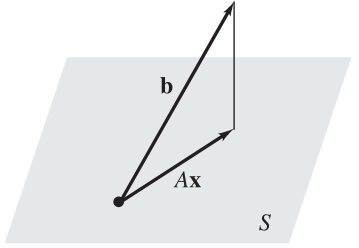
\includegraphics[width = 4cm]{images/leastsquare.png}
    \end{minipage}
    \begin{minipage}{0.6\linewidth}
    Recall that, we are going to find a vector $\B{x}$ that minimize $\norm{A\B{x} - \B{b}}$,
    where $A$ is an $m \x n$ matrix and \B{b} is a column vector in $\R^m$. Let $S$ be the column space of $A$: $S = R(A)$.
    Assume $\B{b} \notin S$, otherwise, the system $A\B{x} = \B{b}$ would be \textit{consistent}.
    \end{minipage}

    From Theorem 5.15, we know that the desired vector is the projection of \B{b} onto $S$.

    Letting $A\hat{\B{x}} = \text{proj}_S\B{b}$ be that projection $\implies A\hat{\B{x}} - \B{b} = \text{proj}_S\B{b} - \B{b}$ is 
    orthogonal to $S = R(A)$.

    This implies that $A\hat{\B{x}} - \B{b} \in  R(A)^\perp$, which equals $N(A^T)$. This is the crucial observation:
    $A\hat{\B{x}} - \B{b}$ is in the \textit{nullspace} of $A^T$.
    \begin{equation*}
        \begin{split}
            A^T (A\hat{\B{x}} - \B{b}) & = \B{0} \\
            A^TA\hat{\B{x}} - A^T\B{b} & = \B{0}\\
            A^TA\hat{\B{x}} & = A^T\B{b}
        \end{split}
    \end{equation*}
    The solution of the least squares problem comes down to solving the $n \x n$ linear S. Eq $A^TA\B{x} = A^T\B{b}$.
    These equations are called the \B{normal equations} of the least squares problem $A\B{x} = \B{b}$.

    \B{Example 7. \textcolor{blue5}{Solving the Normal Equations}}
    Find the solution of the least squares problem 
    \begin{equation*}
        \begin{split}
            A\B{x} & = \B{b} \\
            \begin{bmatrix}
                1 & 1 \\
                1 & 2 \\
                1 & 3
            \end{bmatrix}
            \begin{bmatrix}
                c_0 \\
                c_1
            \end{bmatrix} &= 
            \begin{bmatrix}
                0 \\
                1 \\
                3
            \end{bmatrix}
        \end{split}
    \end{equation*}

    \begin{minipage}{0.3\linewidth}
        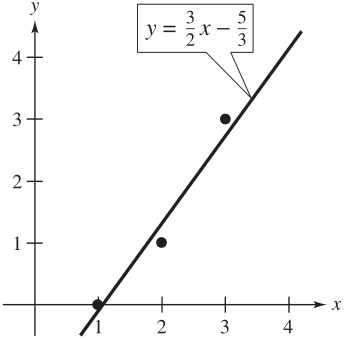
\includegraphics[width = 4cm]{images/normaleq.png}
    \end{minipage}
    \begin{minipage}{0.6\linewidth}
        \T{\textcolor{blue5}{SOLUTION.}} Begin by calculating the matrix products shown below
        \begin{equation*}
            \begin{split}
                A^TA & = \begin{bmatrix}
                    1 & 1 & 1 \\
                    1 & 2 & 3
                \end{bmatrix}
                \begin{bmatrix}
                    1 & 1 \\
                    1 & 2 \\
                    1 & 3
                \end{bmatrix} =
                \begin{bmatrix}
                    3 & 6 \\
                    6 & 14
                \end{bmatrix} \\
                    A^T\B{b} &= \begin{bmatrix}
                    1 & 1 & 1\\
                    1 & 2 & 3
                \end{bmatrix}
                \begin{bmatrix}
                    0 \\ 1 \\ 3
                \end{bmatrix} =
                \begin{bmatrix}
                    4 \\ 11
                \end{bmatrix}
            \end{split}
        \end{equation*}
    \end{minipage}

    The normal equations are
    \begin{equation*}
        \begin{split}
            A^TA\B{x} & = A^T\B{b} \\
            \begin{bmatrix}
                3 & 6 \\
                6 & 14
            \end{bmatrix} 
            \begin{bmatrix}
                c_0 \\ c_1
            \end{bmatrix} & =
            \begin{bmatrix}
                4 \\
                11
            \end{bmatrix}
        \end{split}
    \end{equation*}

    The solution of this system of equations is $\B{x} = \begin{bmatrix}
        -\frac{5}{3} \\
        \frac{3}{2}
    \end{bmatrix}$, which implies that the least squares regression line for the data is $y =\frac{3}{2}x -\frac{5}{3}$.
    
    \B{REMARK.} For an $m \x n$ matrix $A$, the normal equation form an $n \x n$ system of linear equations. This system is
    always consistent, but it may have an \T{infinite number of solutions}. There is a unique solution if the rank of
    $A$ is $n$.

    \B{Example 8. \textcolor{blue5}{Orthogonal Projection onto a Subspace}}
    
    Find the orthogonal projection of the vector $\B{b} = \begin{bmatrix}
        1 \\ 1 \\ 3
    \end{bmatrix}$ onto the column space $S$ of the matrix
    \[ A = \begin{bmatrix}
        0 & 2 \\
        3 & 0 \\
        1 & 0
    \end{bmatrix} \]

    \T{\textcolor{blue5}{SOLUTION.}} 
    \begin{equation*}
        \begin{split}
            A^TA &= \begin{bmatrix}
                0 & 3 & 1 \\
                2 & 0 & 0
            \end{bmatrix}
            \begin{bmatrix}
                0 & 2\\
                3& 0 \\
                1  & 0
            \end{bmatrix} =
            \begin{bmatrix}
                10 & 0 \\
                0 & 4
            \end{bmatrix} \\
                A^T\B{b} &= \begin{bmatrix}
                    0 & 3 & 1 \\
                    2 & 0 & 0
                \end{bmatrix} 
                \begin{bmatrix}
                    1 \\ 1 \\ 3
                \end{bmatrix} = \begin{bmatrix}
                    6 \\ 2
                \end{bmatrix}
        \end{split}
    \end{equation*}
    The normal equations are
    \begin{equation*}
        \begin{split}
            A^TA\B{x} &= A^T\B{b} \\
            \begin{bmatrix}
                10 & 0 \\
                0 & 4
            \end{bmatrix} 
            \begin{bmatrix}
                x_1 \\
                x_2
            \end{bmatrix} &=
            \begin{bmatrix}
                6 \\
                2
            \end{bmatrix}
        \end{split}
    \end{equation*}
    The solution of these equations is $\B{x} = \begin{bmatrix}
        x_1 \\
        x_2
    \end{bmatrix} = \begin{bmatrix}
        \frac{3}{5} \\
        \frac{1}{2}
    \end{bmatrix}$.

    Finally, the projection of $\B{b}$ onto $S$ is
    \[A\B{x} = \begin{bmatrix}
        0 & 2 \\
        3 & 0 \\
        1 & 0
    \end{bmatrix} 
    \begin{bmatrix}
        \frac{3}{5} \\
        \frac{1}{2}
    \end{bmatrix} =
    \begin{bmatrix}
        1 \\
        \frac{9}{5} \\
        \frac{3}{5}
    \end{bmatrix} \]
    which agrees with the solution obtained in \B{Example 5} (find an orthonormal basis of $R(A)$ 
    and applying the formula).

    \subsection{Mathematical Modeling}

    \B{Example 9. \textcolor{blue5}{World Population}}

    \begin{minipage}{0.3\linewidth}
    This table shows \\
    the world population\\
    for 6 different years.     
    \end{minipage}
    \begin{minipage}{0.65\linewidth}
       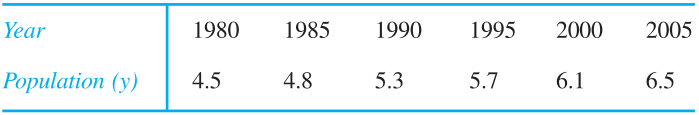
\includegraphics[width = 10cm]{images/population.png}
    \end{minipage}

    Let $x = 0$ represent the year 1980. Find the least squares regression quadratic polynominal
    $y = c_0 + c_1x + c_2x^2$ for these data and use the model to estimate the population for the year 2010.

    \T{\textcolor{blue5}{SOLUTION.}} By substituting the data points $(0, 4.5), (5,4.8), (10, 5.3),
    (15, 5.7), (20, 6.1)$ and $25, 6.5$ into the quadratic polynominal $y = c_0 + c_1x + c_2x^2$, we obtain 
    the following system of linear equations.
    \begin{center}
    \systeme {
        c_0 = 4.5,
        c_0 + 5c_1 + 25c_2 = 4.8,
        c_0 + 10c_1 + 100c_2 = 5.3,
        c_0 + 15c_1 + 225c_2 = 5.7,
        c_0 + 20c_1 + 400c_2 = 6.1,
        c_0 + 25c_1 + 625c_2 = 6.5
    }
    \end{center}
    This produces the least squares problem
    \begin{equation*}
        \begin{split}
            A\B{x} & = \B{b} \\
            \begin{bmatrix}
                1 & 0 & 0 \\
                1 & 5 & 25 \\
                1 & 10 & 100 \\
                1 & 15 & 225 \\
                1 & 20 & 400 \\
                1 & 25 & 625
            \end{bmatrix}
            \begin{bmatrix}
                c_0 \\
                c_1 \\
                c_2
            \end{bmatrix} &=
            \begin{bmatrix}
                4.5 \\
                4.8 \\
                5.3 \\
                5.7 \\
                6.1 \\
                6.5
            \end{bmatrix}
        \end{split}
    \end{equation*}
    The normal equations are
    \begin{equation*}
        \begin{split}
            A^TA\B{x} &= A^T\B{b} \\
            \begin{bmatrix}
                6 & 75 & 1375 \\
                75 & 1375 & 28,125 \\
                1375 & 28,125 & 611,875
            \end{bmatrix}
            \begin{bmatrix}
                c_0 \\
                c_1 \\
                c_2
            \end{bmatrix} &= 
            \begin{bmatrix}
                32.9 \\
                447 \\
                8435
            \end{bmatrix}
        \end{split}
    \end{equation*}
    and their solution is $\B{x} = \begin{bmatrix}
        c_0 \\ c_1 \\ c_2
    \end{bmatrix} \approx \begin{bmatrix}
        4.5 \\
        0.08 \\
        0
    \end{bmatrix}$.

    Note that $c_2 \approx 0$. So, the least squares polynominal for these data is the linear polynominal 
    \[ y = 4.5 + 0.08x \]
    Evaluating this polynominal at $x = 30$ gives the estimate of the world population for the year 2010:
    \[y = 4.5 + 0.08(30) \approx 6.9 \text{ billion } \]

    \B{Example 10. \textcolor{blue5}{Application to Astronomy}}

    \begin{minipage}{0.615\linewidth}
        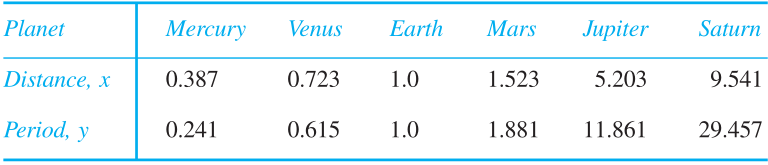
\includegraphics[width = 10cm]{images/planet1.png}
    \end{minipage}
    \begin{minipage}{0.32\linewidth}
        This table shows the mean distances $x$ and the periods $y$ of the 6 planets that are closest to the Sun.
    \end{minipage}

    If you plot the data as the shown, they do not seem to lie in a straight line. By taking the logarithm
    of each coordinate, however, you obtain points of the form $(\ln{x}, \ln{y})$, as below
    \begin{center}
        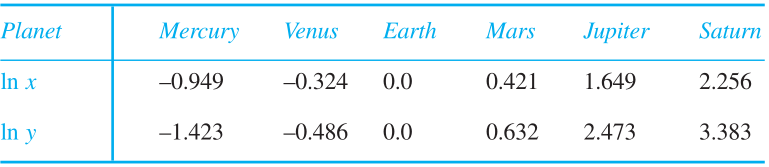
\includegraphics[width = 10cm]{images/planet2.png}
    \end{center}
    \begin{minipage}{0.4\linewidth}
    Using the techniques of this section, we can find the equation of the line is
    \[\ln{y} = \frac{3}{2} \ln{x} \quad \text{or} \quad y = x^{3/2} \]
    \end{minipage}
    \begin{minipage}{0.5\linewidth}
       \begin{flushright}
           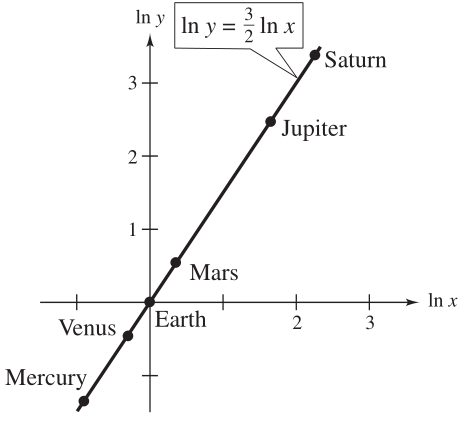
\includegraphics[width = 7cm]{images/planet3.png}
       \end{flushright} 
    \end{minipage}



    \T{MORE EXAMPLE.} (p.351)


    \iffalse
    \begin{equation*}
        \begin{split}

        \end{split}
    \end{equation*}
    \fi
\end{document}
